\documentclass{article}

\def\ParSkip{} 
% Packages
\usepackage{amssymb,amsmath,amsthm,bbm}
\usepackage{verbatim,float,url,dsfont}
\usepackage{graphicx,subfigure,psfrag}
\usepackage{algorithm,algorithmic}
\usepackage{mathtools,enumitem}
\usepackage{multirow}
\usepackage{ragged2e}
\usepackage{xr-hyper}
\usepackage{array}

\usepackage[colorlinks=true,citecolor=blue,urlcolor=blue,linkcolor=blue]{hyperref}
\usepackage[margin=1in]{geometry}
\usepackage[round]{natbib}

\usepackage[utf8]{inputenc} % allow utf-8 input
\usepackage[T1]{fontenc}    % use 8-bit T1 fonts
\usepackage{booktabs}       % professional-quality tables
\usepackage{nicefrac}         % compact symbols for 1/2, etc.
\usepackage{microtype}      % microtypography

\ifdefined\TimesFont 
\usepackage{times} % use times font
\fi

\ifdefined\ParSkip 
\usepackage{parskip} % use par skip
\fi

% Theorems and such
\newtheorem{theorem}{Theorem}
\newtheorem{lemma}{Lemma}
\newtheorem{corollary}{Corollary}
\newtheorem{proposition}{Proposition}
\theoremstyle{definition}
\newtheorem{remark}{Remark}
\newtheorem{definition}{Definition}

% Assumption
\newtheorem*{assumption*}{\assumptionnumber}
\providecommand{\assumptionnumber}{}
\makeatletter
\newenvironment{assumption}[2]{
  \renewcommand{\assumptionnumber}{Assumption #1#2}
  \begin{assumption*}
  \protected@edef\@currentlabel{#1#2}}
{\end{assumption*}}
\makeatother

% Widebar
\makeatletter
\newcommand*\rel@kern[1]{\kern#1\dimexpr\macc@kerna}
\newcommand*\widebar[1]{%
  \begingroup
  \def\mathaccent##1##2{%
    \rel@kern{0.8}%
    \overline{\rel@kern{-0.8}\macc@nucleus\rel@kern{0.2}}%
    \rel@kern{-0.2}%
  }%
  \macc@depth\@ne
  \let\math@bgroup\@empty \let\math@egroup\macc@set@skewchar
  \mathsurround\z@ \frozen@everymath{\mathgroup\macc@group\relax}%
  \macc@set@skewchar\relax
  \let\mathaccentV\macc@nested@a
  \macc@nested@a\relax111{#1}%
  \endgroup
}
\makeatother

% Min and max 
\DeclareMathOperator*{\argmin}{argmin}
\DeclareMathOperator*{\argmax}{argmax}
\DeclareMathOperator*{\minimize}{minimize}
\DeclareMathOperator*{\maximize}{maximize}
\DeclareMathOperator*{\find}{find}
\DeclareMathOperator{\st}{subject\,\,to}

% Other operators
\DeclareMathOperator{\Cov}{Cov}
\DeclareMathOperator{\Var}{Var}
\DeclareMathOperator{\dm}{dim}
\DeclareMathOperator{\col}{col}
\DeclareMathOperator{\row}{row}
\DeclareMathOperator{\nul}{null}
\DeclareMathOperator{\rank}{rank}
\DeclareMathOperator{\nuli}{nullity}
\DeclareMathOperator{\spa}{span}
\DeclareMathOperator{\sign}{sign}
\DeclareMathOperator{\supp}{supp}
\DeclareMathOperator{\diag}{diag}
\DeclareMathOperator{\aff}{aff}
\DeclareMathOperator{\conv}{conv}
\DeclareMathOperator{\dom}{dom}
\DeclareMathOperator{\tr}{tr}
\DeclareMathOperator{\df}{df}

% Other shortcuts 
\def\R{\mathbb{R}}
\def\C{\mathbb{C}}
\def\E{\mathbb{E}}
\def\P{\mathbb{P}}
\def\T{\mathsf{T}}
\def\half{\frac{1}{2}}
\def\df{\mathrm{df}}
\def\hy{\hat{y}}
\def\hf{\hat{f}}
\def\hmu{\hat{\mu}}
\def\halpha{\hat{\alpha}}
\def\hbeta{\hat{\beta}}
\def\htheta{\hat{\theta}}
\def\indep{\perp\!\!\!\perp}
\def\th{^{\textnormal{th}}}

\def\cA{\mathcal{A}}
\def\cB{\mathcal{B}}
\def\cD{\mathcal{D}}
\def\cE{\mathcal{E}}
\def\cF{\mathcal{F}}
\def\cG{\mathcal{G}}
\def\cK{\mathcal{K}}
\def\cH{\mathcal{H}}
\def\cI{\mathcal{I}}
\def\cL{\mathcal{L}}
\def\cM{\mathcal{M}}
\def\cN{\mathcal{N}}
\def\cP{\mathcal{P}}
\def\cS{\mathcal{S}}
\def\cT{\mathcal{T}}
\def\cW{\mathcal{W}}
\def\cX{\mathcal{X}}
\def\cY{\mathcal{Y}}
\def\cZ{\mathcal{Z}}

\usepackage[normalem]{ulem}
\usepackage{centernot}

\title{Lecture 5: Spectral Analysis and Decomposition \\ \smallskip  
\large Introduction to Time Series, Fall 2023 \\ \smallskip
Ryan Tibshirani}
\date{}

\begin{document}
\maketitle
\RaggedRight
\vspace{-50pt}

Related reading: Chapters 4.1--4.3 of Shumway and Stoffer (SS).

\section{Periodic processes}

\begin{itemize}
\item Consider a periodic process of the form 
\begin{equation}
\label{eq:cos_process}
x_t = A \cos(2\pi\omega t + \phi)
\end{equation}

\item Importantly, the quantity $\omega$ in the above definition is called 
  \emph{frequency} of the process; and the quantity $1/\omega$ is called the    
  \emph{period} or \emph{cycle}. As $t$ varies from $0$ to $1/\omega$, note that
  the process goes through one complete cycle (it ends up back where it
  started). See Figure \ref{fig:cos_process} 

\begin{figure}[htb]
\centering
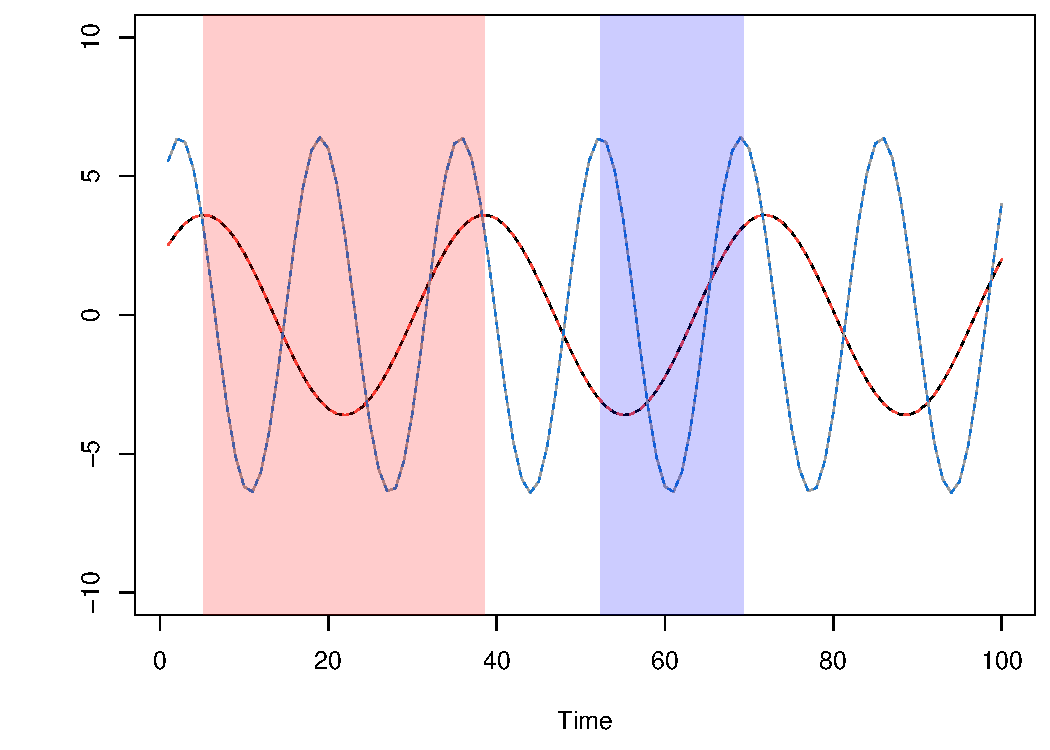
\includegraphics[width=0.85\textwidth]{fig/cos-process-1.pdf}
\caption{Two examples of cosine processes, the first (in red) having a frequency  
  $\omega = 3/100$ and amplitude \smash{$\sqrt{2^2 + 3^2} \approx 3.6$}, and the
  second (in blue) having a frequency $\omega = 6/100$ and amplitude
  \smash{$\sqrt{4^2 + 5^2} \approx 6.4$}.} 
\label{fig:cos_process}
\end{figure}

\item The quantity $A$ is called the \emph{amplitude} and $\phi$ the
  \emph{phase} of the process. The amplitude controls how high the peaks are, 
  and the phase determine where (along the cosine cycle) the process starts at
  the origin $t=0$   

\item We can introduce randomness into the process \eqref{eq:cos_process} by
  allowing $A$ and $\phi$ to be random

\item It will be useful to reparametrize. In general, recall the trigonometric
  identity (cosine compound angle formula):
  \begin{equation}
  \label{eq:compound_angle}
  \cos(a + b) = \cos(a) \cos(b) - \sin(a) \sin(b)
  \end{equation}
  Thus, starting with \eqref{eq:cos_process}, we can rewrite this as $x_t$ = $A
  \cos(\phi) \cos(2\pi\omega t) - A \sin(\phi) \sin(2\pi\omega t)$. Simply
  letting $U_1 = A \cos(\phi)$, $U_2 = -A \sin(\phi)$, we can therefore write   
  \begin{equation}
  \label{eq:cos_sin_process}
  x_t = U_1 \cos(2\pi\omega t) + U_2 \sin(2\pi\omega t)
  \end{equation}
  with $U_1, U_2$ our two random variables, determining the amplitude of the
  cosine and sine components separately

\item Note that another way of writing the relationship between $A,\phi$ and
  $U_1,U_2$ is (why?):
  \[
  A = \sqrt{U_1^2 + U_2^2}, \quad \phi = \tan^{-1}(-U_2/U_1)
  \]

  \item An interesting fact (that you can try to verify as a challenge): 
  \[
  U_1,U_2 \sim N(0,1), \text{ independently} \iff 
  A \sim \chi^2_2, \; \phi \sim \mathrm{Unif}(-\pi,\pi), \text{ independently} 
  \]
\end{itemize}

\subsection{Stationarity}

\begin{itemize}
\item If $U_1,U_2$ are uncorrelated, each with mean zero and variance
  $\sigma^2$, then the periodic process $x_t$, $t = 1,2,3,\dots$ defined in
  \eqref{eq:cos_sin_process} is stationary 

\item To check this: simply compute the mean function
  \[
  \mu_t = \E(x_t) = 0
  \]
  which is constant in time; and the auto-covariance function 
  \begin{align*}
  \gamma(s,t) &= \Cov(x_s, x_t) \\
  &= \Cov\Big( U_1 \cos(2\pi\omega s) + U_2 \sin(2\pi\omega s), \, 
    U_1 \cos(2\pi\omega t) + U_2 \sin(2\pi\omega t) \Big) \\
  &= \Cov\Big( U_1 \cos(2\pi\omega s), \, U_1 \cos(2\pi\omega t) \Big) +
    \Cov\Big( U_2 \sin(2\pi\omega s), \, U_1 \cos(2\pi\omega t) \Big) \\
  &\qquad + \Cov\Big( U_1 \cos(2\pi\omega s), \, U_2 \sin(2\pi\omega t) \Big) +  
     \Cov\Big( U_2 \sin(2\pi\omega s), \, U_2 \sin(2\pi\omega t) \Big) \\
  &=\sigma^2 \cos(2\pi\omega s) \cos(2\pi\omega t) + 0 + 0 + \sigma^2
    \sin(2\pi\omega s) \sin(2\pi\omega t) \\
  &= \sigma^2 \cos(2\pi\omega (s-t))
  \end{align*}
  which only depends on the lag $s-t$ (where in the last line we used the
  identity \eqref{eq:compound_angle} once again)
\end{itemize}

\subsection{General mixtures}

\begin{itemize}
\item As a generalization of \eqref{eq:cos_sin_process}, we can also mix
  together a total of $p$ periodic processes, defining
  \begin{equation}
  \label{eq:cos_sin_process_p}
  x_t = \sum_{i=1}^p \Big( U_{j1} \cos(2\pi\omega_j t) + U_{j2}
  \sin(2\pi\omega_j t) \Big) 
  \end{equation}
  for $U_{j1}, U_{j2}$, $j = 1,\dots,p$ all uncorrelated random variables with
  mean zero, where $U_{j1}, U_{j2}$ have variance $\sigma^2_j$

\item As a generalization of the above calculation, you'll show on your homework
  that the process $x_t$, $t = 1,2,3,\dots$ defined in
  \eqref{eq:cos_sin_process_p} is stationary, with auto-covariance function   
  \[
  \gamma(h) = \sum_{j=1}^p \sigma^2_j \cos(2\pi\omega_j h)
  \]

\item Figure \ref{fig:cos_mixture} displays a couple of mixture processes of the 
  form \eqref{eq:cos_sin_process_p} (with $p=2$ and $p=3$). Note the regular
  repeating nature of the mixture processes. One might wonder how we can
  decompose a such a mixture into its frequency components (periodic processes,
  each of the form \eqref{eq:cos_sin_process}). This is, in fact, one of the
  main objectives in spectral analysis

\begin{figure}[htb]
\centering
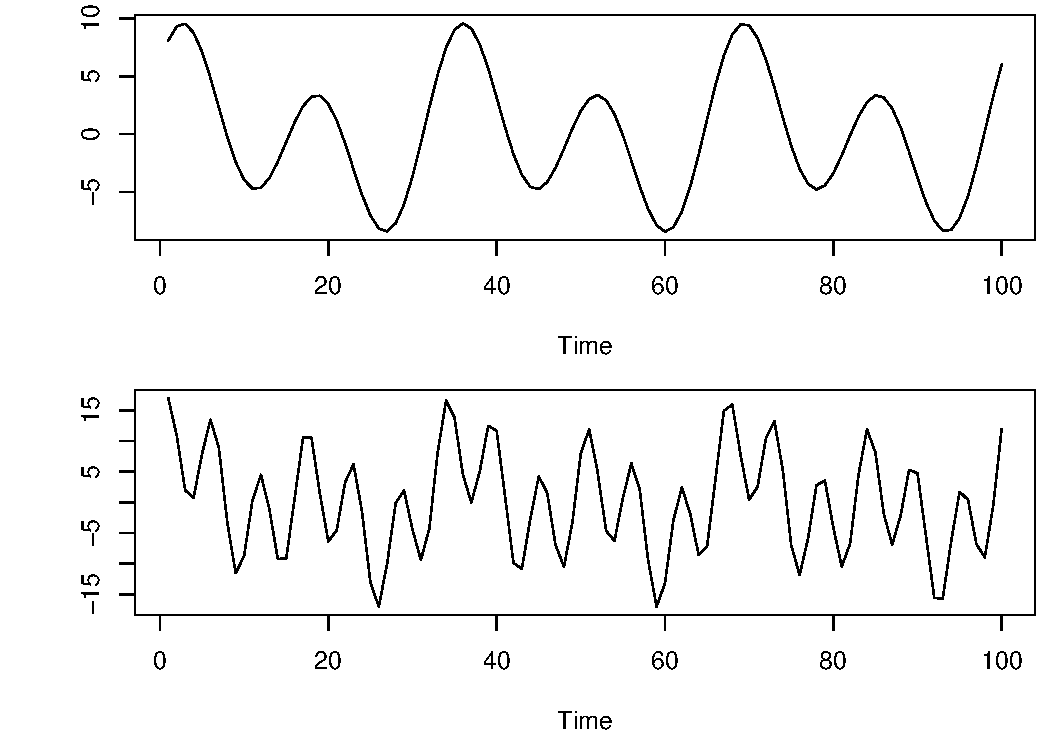
\includegraphics[width=0.85\textwidth]{fig/cos-mixture-1.pdf}
\caption{Mixture of periodic processes of different frequencies (and
  amplitudes).}  
\label{fig:cos_mixture}
\end{figure}

\item And the answer, as we'll see next, is given by something you're already
  quite familiar with ... regression! 
\end{itemize}

\section{Fourier decomposition}

\begin{itemize}
\item Given a time series $x_t$, $t = 1,\dots,n$, consider \emph{seeking} a
  decomposition like \eqref{eq:cos_sin_process_p}. We could do this by
  regressing this time series onto cosine and sine features of different
  frequencies,  
  \begin{align*}
  c_{tj} &= \cos(2\pi j/n \cdot t), \quad t = 1,\dots,n \\
  s_{tj} &= \sin(2\pi j/n \cdot t), \quad t = 1,\dots,n
  \end{align*}
  (which we call these ``basis functions'' in the context of this particular
  regression problem), and so the regression model is 
  \begin{equation}
  \label{eq:fourier_model}
  x_t \approx a_0 + \sum_{j=1}^p (a_j c_{tj} + b_j s_{tj}), \quad t = 1,\dots,n 
  \end{equation}
  Hence the regression coefficients $a_j,b_j$, $j = 1,\dots,p$ represent the 
  amplitudes 

\item How large should $p$ in the above regression model? That is, how many
  cosine and sine basis functions do we need? An amazing fact (at least, it will
  probably seem amazing if you've never seen Fourier decomposition before): 
  \emph{for any time series $x_t$, $t = 1,\dots,n$, we only need to set $p =
    (n-1)/2$, and then the representation in \eqref{eq:fourier_model} will be 
    exact!}  

\item That is, there are coefficients \smash{$\hat{a}_j, \hat{b}_j$}, $j =
  1,\dots,p$ that will give us an equalities in \eqref{eq:fourier_model}, for
  all $t$  

\item (This assumes that $n$ is odd; if $n$ is even, then we need to add an
  additional component $a_{n/2} \cos(\pi t) = a_{n/2} (-1)^t$, and the same
  claim holds: the representation is exact)  

\item To find the coefficients \smash{$\hat{a}_j, \hat{b}_j$}, $j = 1,\dots,p$,
  we can simply perform regresion (least squares). We let $x \in \R^n$ denote
  our time series represented as a vector, which serves as the response vector
  in our regression problem, and we assemble our cosine and sine basis functions
  into a feature matrix  
  \[
  Z = \begin{bmatrix}
  \frac{1}{\sqrt{2n}} & \cos(2\pi \frac{1}{n} \cdot 1) & \sin(2\pi \frac{1}{n}
  \cdot 1) & \cos(2\pi \frac{2}{n} \cdot 1) & \dots & \sin(2\pi \frac{n-1}{2n}
  \cdot 1) \\  
  \frac{1}{\sqrt{2n}}  & \cos(2\pi \frac{1}{n} \cdot 2) & \sin(2\pi \frac{1}{n}
  \cdot 2) & \cos(2\pi \frac{2}{n} \cdot 2) & \dots & \sin(2\pi \frac{n-1}{2n}
  \cdot 2) \\  
  \vdots & & & & & \\
  \frac{1}{\sqrt{2n}}  & \cos(2\pi \frac{1}{n} \cdot n) & \sin(2\pi \frac{1}{n}
  \cdot n) & \cos(2\pi \frac{2}{n} \cdot n) & \dots & \sin(2\pi \frac{n-1}{2n}
  \cdot n)  
  \end{bmatrix} \in \R^{n \times n}
  \]

\item We can then perform regression of $x$ on $Z$ in order to estimate the
  coefficients: 
  \[
  (Z^\T Z)^{-1} Z^\T x
  \]

\item However, something is very special about out matrix $Z$: it satisfies 
  $Z^\T Z = (n/2) I$, where $I$ the $n \times n$ identity matrix. In other
  words, \emph{its columns are uncorrelated, and have squared $\ell_2$ norm
    equal to $n/2$}. This is a very special property of the cosine and sine
  basis functions (and it is the foundation of the discrete Fourier transform, 
  to be discussed shortly)
    
\item Thus, writing $z_j$, $j = 1,\dots,n$ as the columns of $Z$, we have
  \renewcommand{\arraystretch}{1.3} 
  \[
  (Z^\T Z)^{-1} Z^\T x = \begin{bmatrix} \frac{2}{n} z_1^\T x \\ \frac{2}{n}
    z_2^\T x \\ \vdots \\ \frac{2}{n} z_n^\T  x \end{bmatrix},
  \]
 \renewcommand{\arraystretch}{1} 
  so the multiple regression coefficients of $x$ on $Z$ are simply the marginal
  regression coefficients

\item More explicitly, the coefficients are \smash{$\hat{a}_0 = \bar{x}$}, and   
  \begin{equation}
  \label{eq:fourier_coef}
  \begin{aligned}
  \hat{a}_j &= \frac{2}{n} c_j^\T x = \frac{2}{n} \sum_{t=1}^n x_t \cos(2\pi j/n
  \cdot t) \\
  \hat{b}_j &= \frac{2}{n} s_j^\T x = \frac{2}{n} \sum_{t=1}^n x_t \sin(2\pi j/n
  \cdot t) 
  \end{aligned}
  \end{equation}

\item And to be perfectly clear, this gives us the exact decomposition 
  \begin{equation}
  \label{eq:fourier_decomp}
  x_t = \bar{x} + \sum_{j=1}^{(n-1)/2} \Big( \hat{a}_j \cos(2\pi j/n \cdot t) + 
  \hat{b}_j \sin(2\pi j/n \cdot t) \Big), \quad t = 1,\dots,n 
  \end{equation}
  The reason: because $Z$ is orthogonal, it has $n$ linearly independent
  columns in $n$ dimensions, so we can exactly represent any vector as a linear
  combination of its columns---which means that the fitted values from
  regressing $x$ on $Z$ will be exactly $x$  

\item (Side note on computation: at first glance, in order to compute each
  \smash{$\hat{a}_j$} or \smash{$\hat{b}_j$}, we require $O(n)$ operations, and 
  so computing all of them should take $O(n^2$) time ... but in fact the
  \emph{entire set of} coefficients \smash{$\hat{a}_j, \hat{b}_j$}, $j =
  1,\dots,(n-1)/2$ can be computed in $O(n \log{n})$ time using what is known as
  the fast Fourier transform, which we'll return to below)
\end{itemize}

\subsection{Periodogram}

\begin{itemize}
\item Given a series $x_t$, $t = 1,\dots,n$, we can define an object from the
  coefficients \eqref{eq:fourier_coef} in the decomposition
  \eqref{eq:fourier_decomp} that is called the \emph{periodogram}, denoted 
  $P_x$. This takes values at frequencies $j/n$, for $j = 1,\dots,(n-1)/2$, and
  is defined by    
  \begin{equation}
  \label{eq:periodogram}
  P_x(j/n) = \frac{n}{4} \big( \hat{a}_j^2 + \hat{b}_j^2 \big)
  \end{equation}
  When the underlying series is clear from the context, we will drop the
  subscript and simply write $P$ 

\item Large values of the periodogram indicate which frequencies are predominant
  in the given series. This is illustrated in Figure \ref{fig:periodogram_mix},
  which displays the periodogorams for the two series in Figure
  \ref{fig:cos_mixture}. Another nice real data example (from a 1923 texbook on
  numerical analysis!) is given in Figure \ref{fig:periodogram_star}  

\begin{figure}[htb]
\centering
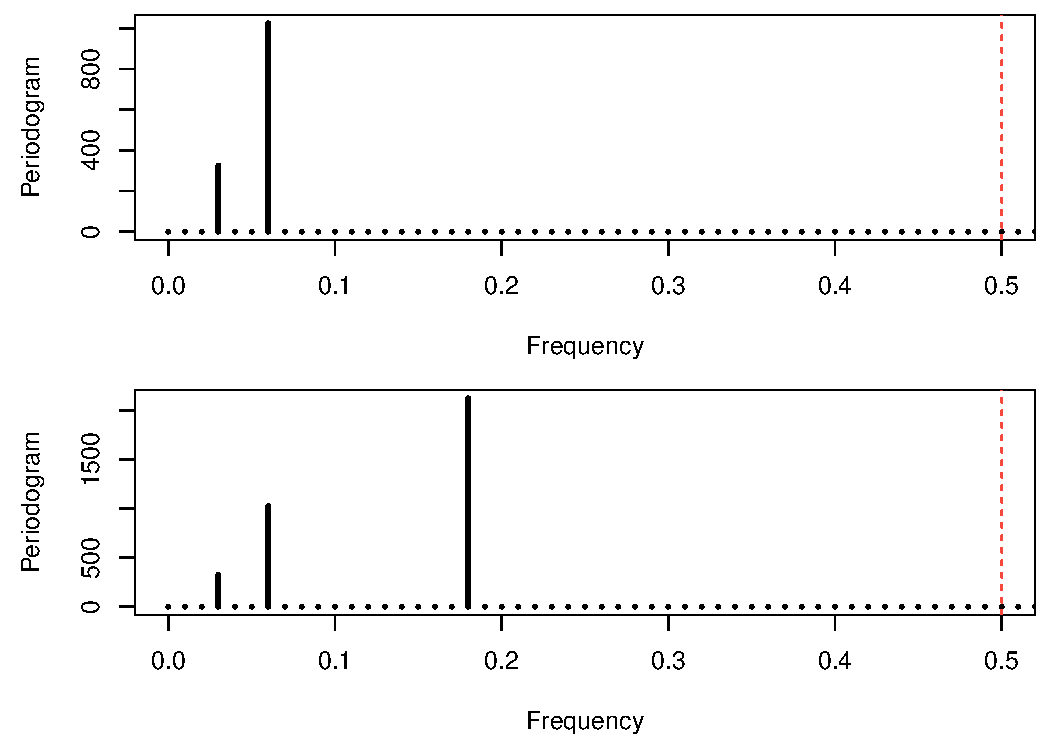
\includegraphics[width=0.85\textwidth]{fig/periodogram-mix-1.pdf}
\caption{Periodograms for the mixture processes in Figure
  \ref{fig:cos_mixture}.} 
\label{fig:periodogram_mix}
\end{figure}

\begin{figure}[htb]
\centering
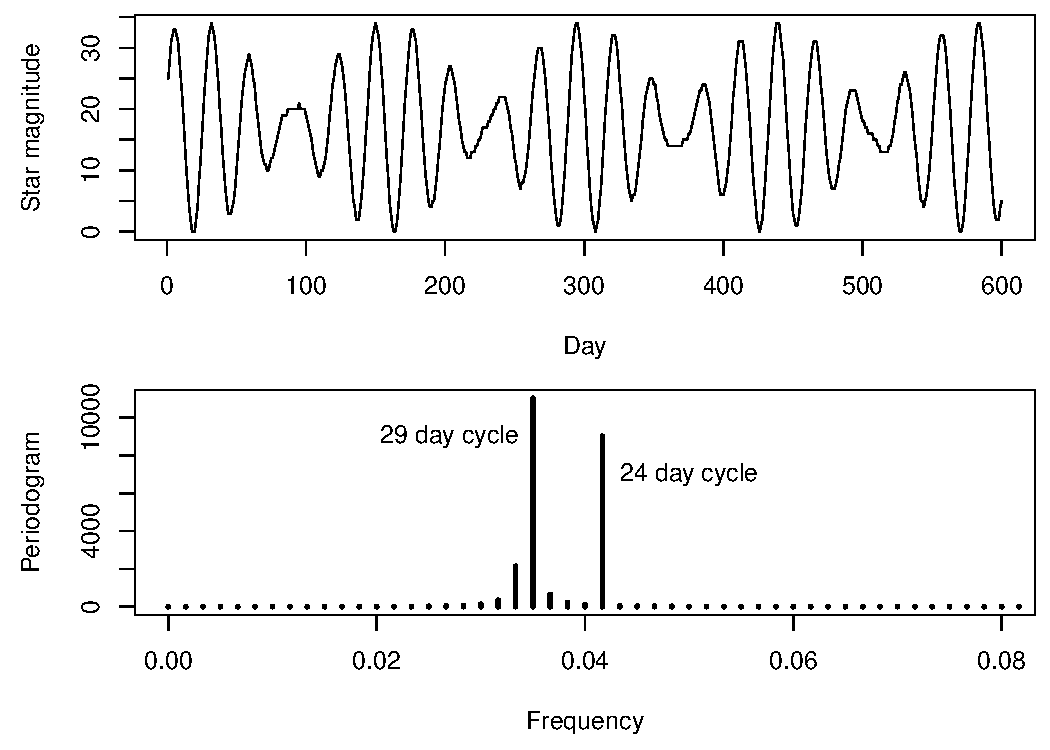
\includegraphics[width=0.85\textwidth]{fig/periodogram-star-1.pdf}
\caption{Periodogram for star magnitude data over 600 consecutive days
  (originally from ``The Calculus of Observations'' by Whittaker and Robinson,   
  adapted by SS). Note the large values of the periodogram at 0.35 and 0.41,
  which correspond to $1/0.35 \approx 29$ and $1/0.41 \approx 24$ day 
  cycles. For more on the interpretation, see Example 4.3 of SS.}
\label{fig:periodogram_star}
\end{figure}

\item If we think back to the mixture process \eqref{eq:cos_sin_process_p} as a
  model for our data, then the periodogram gives us a breakdown of which
  frequencies are the largest \emph{sources of variance}: recall $\sigma_j^2 =
  \E(U_{j1}^2 + U_{j2}^2)/2$ is the variance at frequency $\omega_j$ 
\end{itemize}

\subsection{Discrete Fourier transform}

\begin{itemize}
\item The coefficients \eqref{eq:fourier_coef} used in the decomposition
  \eqref{eq:fourier_decomp} can be computed efficiently by recognizing their
  connection to what is called the \emph{discrete Fourier transform} (DFT) 

\item The DFT of a series $x_t$, $t = 1,\dots,n$, is denoted $d_x$ and defined
  as  
  \begin{equation}
  \label{eq:dft}
  d_x(j/n) = \frac{1}{\sqrt{n}} \sum_{t=1}^n x_t \exp(-2\pi i j/n \cdot t), 
  \quad j = 0,1,\dots,n-1 
  \end{equation}
  where $i$ is the imaginary unit, which satisfies $i^2 = -1$. Thus the DFT is
  complex-value. As before, when the underlying series is clear from the
  context, we will drop the subscript and simply write $d$ 

\item Recalling Euler's formula, $e^{i\theta} = \cos(\theta) + i \sin(\theta)$, 
  we also have (using the fact that cosine is an even function and sine is odd): 
  \[
  d(j/n) = \frac{1}{\sqrt{n}} \sum_{t=1}^n x_t \cos(2\pi j/n \cdot t) - 
  \frac{i}{\sqrt{n}} \sum_{t=1}^n x_t \sin(2\pi j/n \cdot t), \quad j =
  0,1,\dots,n-1   
  \]

\item Thus, from the DFT, we can compute each cosine and sine coefficient in
  \eqref{eq:fourier_coef} by
  \[
  \hat{a}_j = \frac{2}{\sqrt{n}} \mathrm{Re}\{d(j/n)\} \quad \text{and} \quad 
  \hat{b}_j = -\frac{2}{\sqrt{n}} \mathrm{Im}\{d(j/n)\}
  \]
  where for a complex number $z = a+bi$, we use $\mathrm{Re}\{z\} = a$ and
  $\mathrm{Im}\{z\} = b$ to denote its real and imaginary parts

\item Note the following interesting connection to the periodogram. Since the
  the modulus of each entry of the DFT satisfies (by definition) $|d(j/n)|^2 = 
  \mathrm{Re}\{d(j/n)\}^2 + \mathrm{Im}\{d(j/n)\}^2$, the periodogram in
  \eqref{eq:periodogram} is 
  \begin{align}
  \nonumber
  P(j/n) &= \frac{n}{4} \big( \hat{a}_j^2 + \hat{b}_j^2 \big) \\
  \nonumber
  &= \frac{n}{4} \bigg( \frac{4}{n} \mathrm{Re}\{d(j/n)\}^2 +
    \frac{4}{n} \mathrm{Im}\{d(j/n)\}^2 \bigg) \\
  \label{eq:periodogram_dft}          
  &= |d(j/n)|^2
  \end{align}

\item In other words, the periodogram is simply the squared modulus of the DFT! 

\item Side note: the entire DFT can be computed rapidly using an algorithm
  called the fast Fourier transform (FFT), which takes $O(n\log{n})$ operations 
  (most efficient in practice when $n$ is a highly composite integer, such as a
  power of 2). The modern generic FFT algorithm is credited to Cooley and Tukey
  in the 1960s, but similar ideas were arround much earlier   

\item Side side note: different software implementations scale the FFT/DFT 
  differently, so you have to be careful to consult the documentation. For
  example, the \verb|fft()| function in R computes it without the leading factor
  of $n^{-1/2}$, and with an additional factor of $\exp(2\pi i j/n)$, but this
  doesn't matter since we're only using it in our examples to compute the
  squared modulus, i.e., the periodogram, across frequencies
\end{itemize}

\section{Interlude: ST decomposition}

\begin{itemize}
\item As an interlude, we'll demo how to use the periodogram, in combination
  with smoothing (as we learned in the last lecture) to detect the presence of 
  seasonality in time series, and fit a seasonal-trend (ST) decomposition 

\item Warning: what we do here is very simple and may very well offend
  researchers well-versed in classical time series decomposition and
  econometrics alike. It is only meant as a demo. We repeat: it is just a demo! 

\item (You can learn more about decomposition methods in time series in Chapters 
  3.4--3.6 of the HA book. It is worth mentioning that in statistics, the STL
  decomposition is pretty standard and popular, which stands for
  ``seasonal-trend decomposition using LOESS'', with LOESS being a particular
  type of smoother that we didn't cover, but it acts like kernel smoother with a
  varying bandwidth. For an econometrics perspective, see the references from
  the last lecture: Hodrick-Prescott $\to$ Hamilton $\to$ Hodrick again. The
  last reference is especially scholarly and reviews what has been done over the
  years)

\item Ok with all those caveats laid out, a pretty simple and generic method to
  perform an ST decomposition of a time series $y_t$, $t = 1,\dots,n$ is as
  follows:    
  \begin{itemize}
  \item Use a smoother to estimate a trend \smash{$\htheta_t$}, $t = 1,\dots,n$,
    aiming to undersmooth somewhat so as to ignore a (possible) cyclic or
    seasonal component 

  \item Compute residuals \smash{$r_t = y_t - \htheta_t$}, $t = 1,\dots,n$

  \item Absent any prior knowledge about the periods of the seasonal component 
    (i.e., without wanting to specify a priori that there might be weekly,
    monthly, quarterly, etc. components), just compute the periodogram of the
    residuals

\item Identify large peaks in the periodogram, and fit and add to the model
  seasonal components that correspond to the predominant periods (inverse 
  frequencies) that are present  
  \end{itemize}

\item Of course the method presented above is limited in several ways (e.g., it
  assumes that the seasonal components have constant amplitude over time), and
  other methods are more advanced in various ways. You can read more in the 
  aforementioned references if you are curious

\item Figure \ref{fig:st_decomposition} gives an example applied to US retail 
  employment data. We can see very clear cycles at about a year, half-year,
  third-year, and quarter-year 

\begin{figure}[htb]
\centering
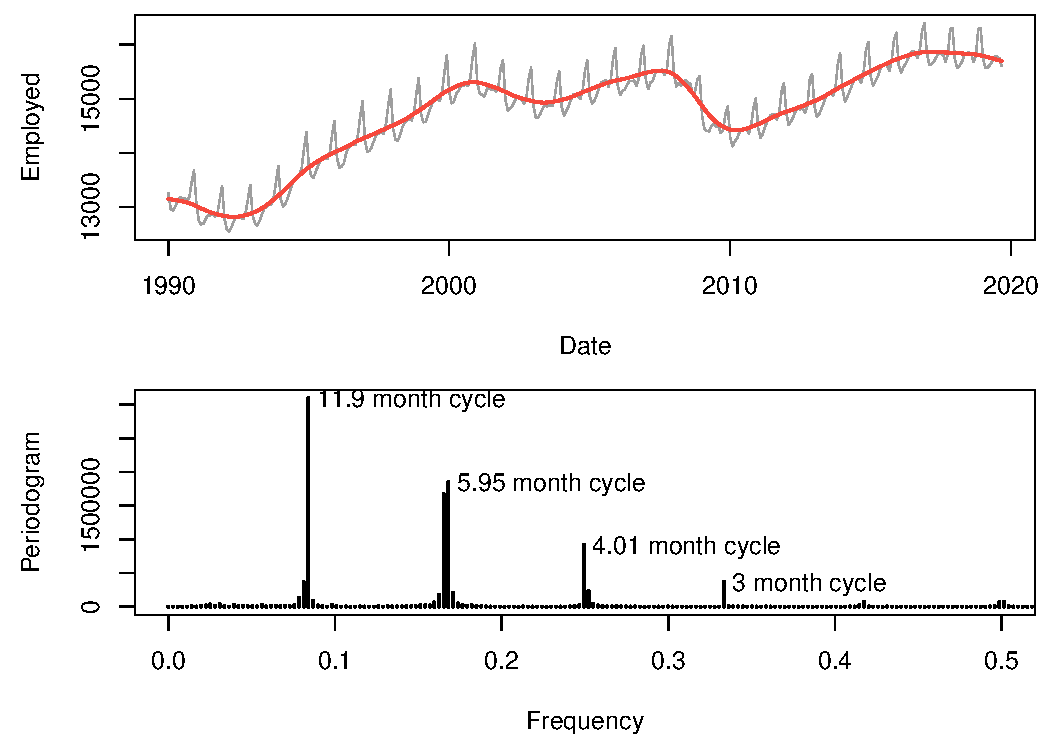
\includegraphics[width=0.85\textwidth]{fig/st-decomposition-1.pdf}
\caption{ST decomposition, using an HP filter for the smoother, and a
  periodogram on the residuals to detect predominant frequency components.}  
\label{fig:st_decomposition}
\end{figure}
\end{itemize}

\section{Spectral representation}

\begin{itemize}
\item Now we turn to a general fact about stationary processes in time series,
  which is called the spectral representation of the auto-covariance function 

\item In particular, if $x_t$, $t = 1,2,3,\dots$ is stationary with
  auto-covariance function $\gamma(h) = \Cov(x_{t+h}, x_t)$, then there exists a 
  unique increasing function $F$, called the \emph{spectral distribution
    function} corresponding to the process, with $F(\omega) = 0$ for $\omega
  \leq -1/2$, and $F(\omega) = \gamma(0)$ for $\omega \geq 1/2$, such that for
  any $h = 0, \pm 1, \pm 2, \dots$,  
  \[
  \gamma(h) = \int_{-1/2}^{1/2} \exp(2\pi i \omega h) \, dF(\omega) 
  \]

\item Above, we can think of $F$ as being analogous to a cumulative distribution
  function (CDF), and thus the integral as being analogous as an expectation
  defined with respect the distribution that governs $F$. The only difference is
  that the total mass here of need not be 1, but is instead $\gamma(0)$ 

\item We will generally ignore this distinction and call $F$ a distribution
  anyway, and in the case $F$ is differentiable, we will denote its derivative
  by $f$ and call this the \emph{spectral density}

\item When the spectral density exists,\footnote{It exists when the
    auto-covariance function is absolutely summable, which means that it
    satisfies \smash{$\sum_{h=-\infty}^\infty |\gamma(h)| < \infty$}. See
    Appendix C of SS for details.} 
  note that we have the representation 
  \[
  \gamma(h) = \int_{-1/2}^{1/2} \exp(2\pi i \omega h) \, f(\omega) \, d\omega,
  \quad h = 0, \pm 1, \pm 2, \dots
  \]

\item There is also an inverse relationship: we can represent $f$ in terms of
  $\gamma$, via 
  \begin{equation}
  \label{eq:spectral_density}
  f(\omega) = \sum_{h=-\infty}^\infty \gamma(h) \exp(-2\pi i \omega h), \quad
  \omega \in [-1/2, 1/2] 
  \end{equation}
  In other words, the spectral density and auto-covariance function are
  \emph{Fourier transform} pairs

\item The important high-level perspective to remember here: \emph{the
    auto-covariance function and spectral density contain the same information 
    about a time series, but express it in different ways}

\item The auto-covariance function expresses the variation broken down by
  \emph{lags}, whereas the spectral density expresses variation broken down by
  \emph{frequencies}---or by \emph{cycles} (remembering that the inverse of a
  frequency is a cycle)  

\item Next we compute the spectral density in a number of our favorite example
  stationary time series models. It will be helpful to point out that $\gamma(h)
  = \gamma(-h)$ implies $f(\omega) = f(-\omega)$, so we only need to keep track
  of $f$ for $\omega \in [0, 1/2]$ 
\end{itemize}

\subsection{White noise}

\begin{itemize}
\item Recall our most basic stationary process which is white noise: $x_t$, $t = 
  1,2,3,\dots$ are uncorrelated random variables, with zero mean, and constant 
  variance $\sigma^2$. So
  \[
  \gamma(h) = \begin{cases} 
    \sigma^2 & h = 0 \\
    0 & h \not= 0
  \end{cases}
  \]
 
\item The spectral density, according to \eqref{eq:spectral_density}, is
  therefore
  \[
  f(\omega) = \sigma^2, \quad \omega \in [0, 1/2]
  \]

\item So, white noise has the simplest spectral density there is: it is constant! 

\item For the moment you (may) have been waiting for: we can finally explain
  where a lot of the nomenclature is coming from ... if we think about a time
  series as being comprised of a mixture of colors---which we can generally do
  since any time series has the periodic representation
  \eqref{eq:fourier_decomp}---then \emph{spectral analysis} provides us a tool
  like a prism, for decomposing this series into its primary colors, or
  \emph{spectra}. And, just like the color white, a \emph{white noise} series is
  an equal mix of all colors (frequencies)
\end{itemize}

\subsection{MA model}

\begin{itemize}
\item Moving on to a moving average: consider $x_t = w_t + \theta w_{t-1}$, $t =
  1,2,3,\dots$, where $w_t$, $t = 1,2,3,\dots$ is a white noise sequence. The
  right-hand side here is not exactly the same as an equal-weights moving
  average (as we've looked at many times before), but a linear filter of the
  past, with weights $a_0 = 1$ and $a_1 = \theta$. It is generally what we'll
  call a moving average (MA) model in the context of ARIMA, as we'll learn soon  

\item By direct calculation, which you can check, the auto-covariance function
  is: 
  \[
  \gamma(h) = \begin{cases}
  (1+\theta^2) \sigma^2 & h = 0 \\
  \theta^2 \sigma^2 & |h| = 1 \\
  0 & |h| > 1 \\
  \end{cases}
  \]
  where $\sigma^2$ denotes the variance of $w_t$

\item The spectral density, according to \eqref{eq:spectral_density}, is
  therefore
  \begin{align*}
  f(\omega) &= (1+\theta^2) \sigma^2 + \theta^2 \sigma^2 (e^{2\pi i \omega} +
              e^{-2\pi i \omega}) \\
  &=  \sigma^2 \Big( 1+\theta^2 + 2 \theta^2 \cos(2\pi \omega) \Big)
  \end{align*}
  where in the second line we used $\cos(\theta) = (e^{i\theta} +e^{i\theta}) / 
  2$, which follows from Euler's formula $e^{i\theta} = \cos(\theta) + i
  \sin(\theta)$

\item So an MA process has a spectral density that decays from zero, and larger
  $\theta$ means a steeper decay from $\omega = 0$ to $\omega = 1/2$. See Figure
  \ref{fig:spectral_density_ma} for an illustration  

\begin{figure}[htb]
\centering
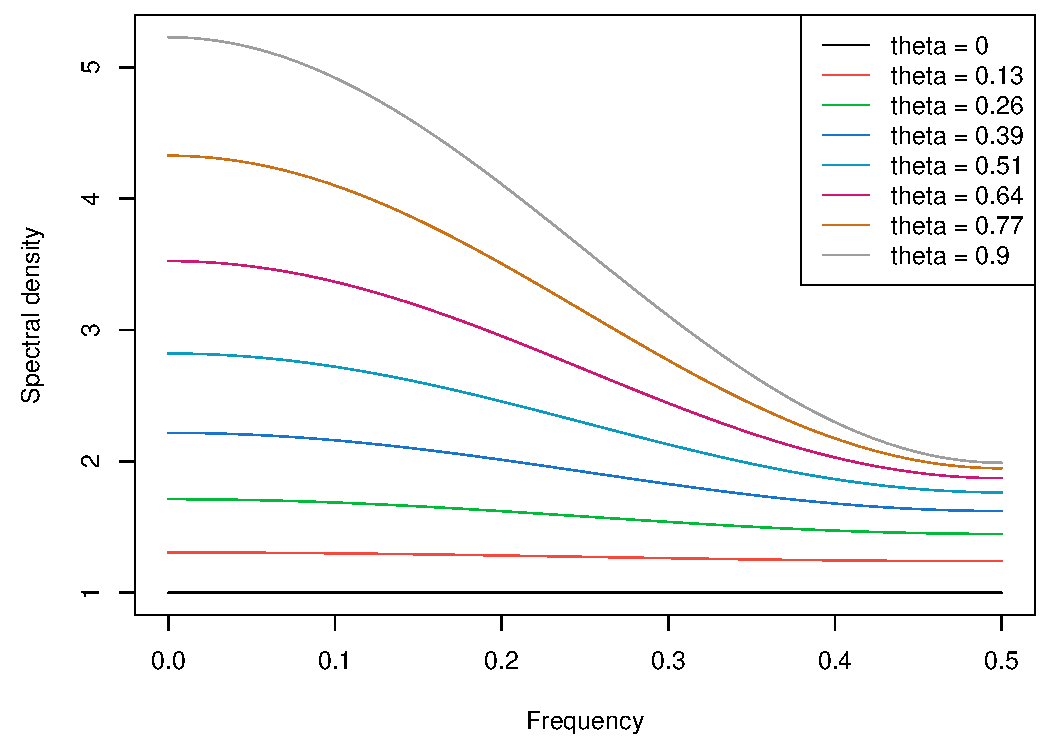
\includegraphics[width=0.85\textwidth]{fig/spectral-density-ma-1.pdf}
\caption{Spectral density for the MA model, as $\theta$ varies.}
\label{fig:spectral_density_ma}
\end{figure}
\end{itemize}

\subsection{AR model}

\begin{itemize}
\item Lastly, we'll turn to an autoregressive model: consider $x_t = \phi_1
  x_{t-1} + \phi_2 x_{t-2} + w_t$, $t = 1,2,3,\dots$, where $w_t$, $t = 
  1,2,3,\dots$ is a white noise sequence. This is a second-order autoregressive
  (AR) model, which we'll learn more about when we cover ARIMA soon

\item Calculating the auto-covariance function is going to a bit nasty for this 
  process (as you'll learn more about later when we cover ARIMA). However, for
  our purposes here, we can get away with a trick: finding an equation that
  relates the auto-covariance of white noise tot hat of the AR process 

\item Since $w_t = x_t - \phi_1 x_{t-1} - \phi_2 x_{t-2}$, $t = 1,2,3,\dots$, we
  have 
  \begin{align*}
  \gamma_w(h) &= \Cov(w_{t+h}, w_t) \\
  &= \Cov(x_{t+h} - \phi_1 x_{t+h-1} -  \phi_2 x_{t+h-2}, \,
    x_t - \phi_1 x_{t-1} - \phi_2 x_{t-2}) \\
  &= \gamma_x(h) - \phi_1 \gamma_x(h+1) - \phi_2 \gamma_x(h+2) 
    - \phi_1 \gamma_x(h-1) + \phi_1^2 \gamma_x(h) + \phi_1 \phi_2 
    \gamma_x(h+1) \\ 
    &\qquad - \phi_2 \gamma_x(h-2) +  \phi_1 \phi_2 \gamma_x(h-1) + \phi_2^2
    \gamma_x(h) \\
    &= (1+\phi_1^2+\phi_2^2) \gamma_x(h)  
      -\phi_1(1-\phi_2) \big( \gamma_x(h-1) + \gamma_x(h+1) \big) 
      - \phi_2 \big( \gamma_x(h-2) + \gamma_x(h+2) \big)  
  \end{align*}

\item Now represent the auto-covariance function $\gamma_x$ as an integral with
  respect to the spectral density $f_x$:
  \[
  \gamma_w(h) = \int_{-1/2}^{1/2} \Big( (1+\phi_1^2+\phi_2^2)  
  - \phi_1(1-\phi_2) (e^{-2\pi i \omega} + e^{2\pi i \omega})
  - \phi_2 (e^{-4\pi i \omega} + e^{4\pi i \omega}) \Big) \exp(2\pi i \omega
  h) \, f_x(\omega) \, d\omega
  \]

\item However, note that the representation of $\gamma_w$ in terms of its own
  spectral density $f_w$ is of course
  \[
  \gamma_w(h) = \int_{-1/2}^{1/2} \exp(2\pi i \omega h) \, f_w(\omega) \,
  d\omega 
  \]

\item Since Fourier transforms are uniquely identifying, we infer that the
  integrands in the last two display must match:
  \[
  \Big( (1+\phi_1^2+\phi_2^2)  
    - \phi_1(1-\phi_2) (e^{-2\pi i \omega} + e^{2\pi i \omega})
    - \phi_2 (e^{-4\pi i \omega} + e^{4\pi i \omega}) \Big) \exp(2\pi i \omega
    h) \, f_x(\omega) = f_w(\omega)
  \]

\item And based on our earlier calculation for white noise, we know that
  $f_w(\omega) = \sigma^2$, the noise variance, so plugging that into the above,
  we learn 
  \begin{align*}
  f_x(\omega) &= \frac{\sigma^2}{ (1+\phi_1^2+\phi_2^2)  
    - \phi_1(1-\phi_2) (e^{-2\pi i \omega} + e^{2\pi i \omega})
    - \phi_2 (e^{-4\pi i \omega} + e^{4\pi i \omega}) } \\
  &= \frac{\sigma^2}{ (1+\phi_1^2+\phi_2^2)  
    -2 \phi_1(1-\phi_2) \cos(2\pi \omega) 
    - 2 \phi_2 \cos(4\pi \omega) }
  \end{align*}
  where in the second line we used the identity $\cos(\theta) = (e^{i\theta}
  +e^{i\theta}) / 2$ once again

\item Plotting this, as we do in Figure \ref{fig:spectral_density_ar}, we learn
  that a second-order AR process has a spectral density that is concentrated
  around a particular frequency. For example, when $\phi_1 = 1$ and $\phi_2 = 
  -0.9$, it is concentrated around $\omega \approx 0.16$ (a cycle of $1/\omega
  \approx 6$ time points)

\begin{figure}[htb]
\centering
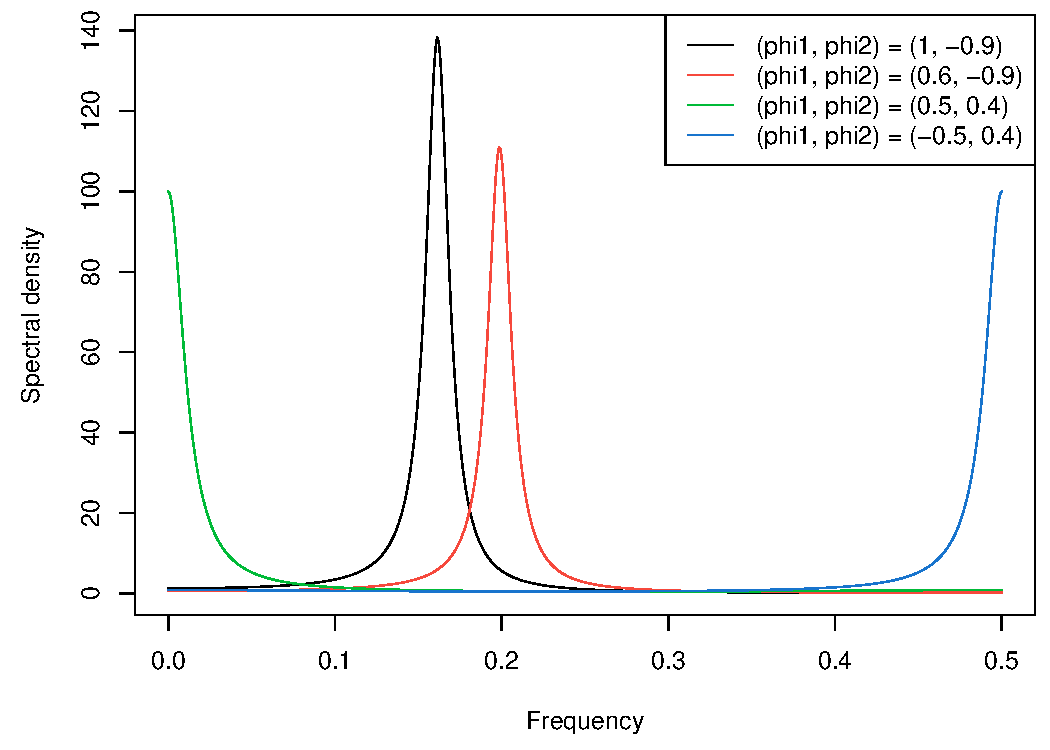
\includegraphics[width=0.85\textwidth]{fig/spectral-density-ar-1.pdf}
\caption{Spectral density for the second-order AR model, for a few parameter
  choices $\phi_1,\phi_2$.}
\label{fig:spectral_density_ar}
\end{figure}
\end{itemize}

\subsection{Sample spectral density}

\begin{itemize}
\item To conclude, let's draw a connection between the two main players that
  we've seen in this lecture: the periodogram, and the spectral density 

\item Recall the DFT \eqref{eq:dft} of a series $x_t$, $t = 1,\dots,n$, which we
  can rewrite as
  \[
  d(\omega_j) = \frac{1}{\sqrt{n}} \sum_{t=1}^n x_t \exp(-2\pi i \omega_j t) 
  \]
  for $\omega_j = j/n$, $j = 0,1,\dots,n-1$

\item We claim that \smash{$\sum_{t=1}^n \exp(-2\pi i \omega_j t) = 0$}
  for any $j < n$. This can be check by viewing it as a geometric series
  \smash{$\sum_{t=1}^n z^t$} in $z = e^{2\pi i j / n}$, and hence we can use the
  formula  
  \[
  \sum_{t=1}^n z^t = z \frac{1-z^n}{1-z}, \quad \text{for $z \not= 1$}
  \] 
  but here $z^n = e^{2\pi i j} = 1$ for any $j < n$

\item Using the last fact, we can thus rewrite the DFT once more as  
  \[
  d(\omega_j) = \frac{1}{\sqrt{n}} \sum_{t=1}^n (x_t - \bar{x}) \exp(-2\pi i
  \omega_j t)
  \]

\item The periodogram, recalling \eqref{eq:periodogram_dft}, is given by the 
  squared modulus of the DFT, $P(\omega_j) = |d(\omega_j)|^2$. Using the fact
  that the squared modulus of $z = a+bi$ is $|z|^2 = a^2 + b^2 = (a+ib)(a-ib)$,  
  \begin{align*}
  P(\omega_j) &= \frac{1}{n} \sum_{s=1}^n \sum_{t=1}^n (x_s - \bar{x}) (x_t -
    \bar{x}) \exp\big( -2\pi i \omega_j (t-s) \big) \\
  &= \frac{1}{n} \sum_{h=-(n-1)}^{n-1} \sum_{t = s+h} (x_s - \bar{x}) (x_{s+h} -
    \bar{x}) \exp(-2\pi i \omega_j h) \\
  &= \sum_{h=-(n-1)}^{n-1} \frac{1}{n} \sum_{s=1}^{n-|h|} (x_s - \bar{x})
    (x_{s+|h|} - \bar{x}) \exp(-2\pi i \omega_j h) \\
  &= \sum_{h=-(n-1)}^{n-1} \hat\gamma(h) \exp(-2\pi i \omega_j h)
  \end{align*}
  where \smash{$\hat\gamma(h)$} is our usual sample auto-covariance at lag $h$ 

\item Compare the last line to the spectral density \eqref{eq:spectral_density},
  and what do you find? The periodogram is simply a \emph{sample spectral
    density} estimator, at discrete frequencies $\omega_j$, $j = 0,\dots,n-1$ 

\item For models in which we expect smoothness in the spectral density, the
  sample spectral density (periodogram) turns out to be not such a good
  estimator. There is much more we can do, and much more to say about spectral
  analysis and filtering in general. See Chapters 4.4--4.10 of the SS book if
  you're interested in learning more
\end{itemize}
\end{document}
